\chapter{Trattamento dei segnali elettrici}
\section{Impedenze}
Tipicamente uno strumento possiede un alta impedenza di ingresso, per non perturbare il segnale e una bassa impedenza in uscita,
per minimizzare la perdita di segnale.\\
L'unica eccezione \`e data dai segnali veloci, dove problemi legati alla riflessione del segnale richiedono l'uso di impedenze adattate,
in questo caso si avr\`a attenuazione del segnale per non avere deformazioni nell'impulso.
\section{Effetto pelle}
L'effetto pelle \`e l'effetto per cui una corrente elettrica alternata tende a scorrere maggiormente lungo la superficie di un conduttore rispetto
alle regioni interne.
Il motivo di questo effetto \`e legato ai campi magnetici interni variabili (per via della corrente alternata) e quindi a correnti
indotte che impediscono il fluire della corrente all'interno del cavo.\\
Il risultato di questo fenomeno \`e un aumento della resistenza del conduttore al crescere della frequenza del segnale elettrico,
in quanto una parte del conduttore non viene utilizzata.
\section{I cavi coassiali}
Sono cavi schermati da una maglia di rame, essa funge da schermo per le interferenze a bassa e altissima frequenza (sopra i 100 kHz).
Non \`e un ottimo schermo per le frequenze intermedie (\textbf{approfondire}): in questo caso si usano cavi a doppia schermatura,
oppure si fanno passare i cavi dentro un tubo di materiale conduttore.\\
La velocit\`a di trasmissione del segnale nel cavo tipica \`e circa il 66\% di $c$, tuttavia esistono speciali cavi ritardanti dove
la velocit\`a pu\`o arrivare al 1\%; la velocit\`a \`e proporzionale a $Z = \sqrt{\frac{L}{C}}$.\\
In un cavo le \textbf{caratteristiche fondamentali} sono l'impedenza, l'induttanza e la capacit\`a per unit\`a di lunghezza.
Se il cavo deve trasportare l'alta tensione, allora \`e importante la massima tensione trasportabile.\\
\subsection{Disturbi nei coassiali}
Ogni cavo \`e soggetto a perdite dissipative legate alla resistenza del conduttore, esse sono trascurabili per lunghezze fino a qualche
decina di metri, salvo per impulsi con tempi di salita molto brevi.
Ad esempio un segnale con fronte di salita di 1 ns subisce evidenti distorsioni anche solo con cavi lunghi 3 m, per via di effetti di
riflessione dell'impulso.\\
La schermatura viene anche utilizzata serve per fare da riferimento di massa comune tra i vari dispositivi e viene connesso allo
chassis del dispositivo, ovvero l'involucro metallico dell'apparecchio.\\
Un effetto che \`e importante evitare \`e il \textbf{ground loop} (\textbf{approfondire}):
se il riferimento di massa fa una forma chiusa, per garantire un potenziale comune pu\`o circolare una corrente continua.
Questa corrente pu\`o subire fluttuazioni che generano correnti spurie nel mio segnale, disturbandolo.
Per evitare questo effetto, \`e importante che ogni strumento abbia un riferimento interno di massa, che l'alimentazione venga fornita
a stella da un unico distributore, che la massa degli strumenti coincida con quella dell'alimentatore e che la corrente venga prelevata
da una sola presa con un circuito dedicato.\\
Segnali di transiente di accensione/spegnimento di un dispositivo possono indurre correnti nella schermatura del coassiale,
provocando disturbi. 
Ad esempio i monitor dei computer introducono importanti disturbi ad alta frequenza.\\
\subsection{Metodi di abbattimento del rumore}
Per abbattere il rumore si pu\`o utilizzare un amplificatore operazionale in configurazione differenziale:
il cavo che trasporta il segnale viene intrecciato con un cavo non connesso al dispositivo, il secondo cavo serve per sondare i disturbi
ambientali a cui \`e soggetto il primo, in questo modo il preamplificatore pu\`o eliminare i disturbi comuni e pulire il segnale in gran parte (\textbf{approfondire}).
\subsection{Impedenza caratteristica e riflessione del segnale}
Nella trasmissione di segnali ci si riferisce a due casi limite:
\begin{itemize}
\item Segnali lenti o a bassa frequenza
\item Segnali veloci o ad alta frequenza
\end{itemize}
Tipicamente in un coassiale la velocit\`a di trasmissione di un segnale e 5 ns/m, se il \textit{risetime} del segnale \`e maggiore del tempo
di salita si parla di segnali \textbf{lenti}, altrimenti parliamo di segnali veloci (ad esempio succede nei segnali provenienti dagli scintillatori plastici.
\textbf{Su cavi lunghi centinaia di metri i segnali provenienti da rivelatori sono veloci.}
\subsubsection{Segnali lenti o a bassa frequenza}
Per i segnali lenti la resistenza serie del cavo \`e trascurabile, purch\'e la lunghezza del cavo non superi le centinaia di metri.\\
La capacit\`a verso massa \`e 50-100 pf/m, questa capacit\`a deve essere la pi\`u piccola possibile, in quanto si somma a quella del rivelatore;
l'ampiezza del segnale misurato \`e inversamente proporzionale a C, per quest\`o \`e importante avere cavi corti.
\subsubsection{Segnali veloci o ad alta frequenza}
\`E fondamentale considerare l'\textbf{impedenza caratteristica}: essa \`e dipendente dal dielettrico e dal diametro del conduttore centrale
e dello schermo, mentre non \`e dipendente dalla lunghezza (essa dipende dal rapporto tra induttanza e capacit\`a per unit\`a di lunghezza del cavo).
L'impedenza caratteristica \`e pari all'impedenza con la quale bisogna chiudere il cavo per poter trasmettere impulsi di tensione senza
avere effetti di riflessione del segnale.\\
Tipicamente se si chiude il cavo con un impedenza infinita si osserva riflessione totale di segnale senza sfasamenti,
mentre se si chiude il cavo con un impedenza nulla si osserva una riflessione totale, ma di verso opposto.
Quando si attacca la strumentazione il cavo vede come resistenza di terminazione la resistenza di ingresso dello strumento.
Tenendo conto che gli strumenti hanno, in generale, una resistenza di ingresso alta si deduce che in presenza di segnali veloci si osservano effetti
di riflessione (l'impedenza tipica di un cavo coassiale \`e 50 $\Omega$.
Per questo motivo quando si lavora in queste condizioni si termina il cavo con una resistenza di shunt di valore pari alla resistenza caratteristica.
Il cavo vede questa resistenza in parallelo con quella di ingresso del dispositivo: essendo quest'ultima molto maggiore dell'impedenza caratteristica
la resistenza vista diventa pari alla resistenza di shunt.\\
\`E importante tenere conto del fatto che spesso i dispositivi studiati per lavorare appositamente con segnali veloci hanno gi\`a una resistenza di ingresso di 50 $\Omega$,
per cui \`e importante verificare questo fatto.
\section{Attenuatori di segnali}
Talvolta i segnali elettrici sono troppo intensi, per questo diventa necessario ricorrere a degli attenuatori di segnale.\\
L'attenuatore pi\`u semplice che si possa pensare \`e un \textbf{partitore di tensione}, tuttavia questa tecnica porta ad avere problemi
di disturbi con segnali ad alta frequenza.\\
Un altro attenuatore utilizzato \`e l'attenuatore a T (figura~\ref{fig:attenuatoreT}), in questo attenuatore la resistenza di uscita $R_0$
pu\`o essere accoppiata con l'impedenza del cavo e ponendo $\alpha=V_i/V_o$  con le resistenze:
\begin{equation*}
R_1 = R_o \frac{\alpha - 1}{\alpha + 1}
\end{equation*}
e
\begin{equation*}
R_2 = R_o \frac{2 \alpha}{\alpha^2 - 1}
\end{equation*}
si ha l'attenuazione desiderata.
\begin{figure}[htbp]
\begin{center}
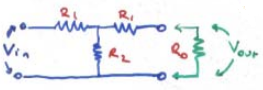
\includegraphics[scale=1]{./Immagini/AttenutatoreT.png}
\caption{Un attenuatore a T}
\label{fig:attenuatoreT}
\end{center}
\end{figure}
\section{Sdoppiamento del segnale}
Per sdoppiare i segnali lenti \`e possibile usare una T semplice, per i segnali ad alta frequenza \`e necessario prendere qualche accorgimento
aggiuntivo, la figura~\ref{fig:sdoppiatore} mostra come deve essere realizzato lo sdoppiamento:
le resistenze R sono da 16.6 $\Omega$ e vengono poste una per ogni ramo dello sdoppiamento.
Inoltre viene posto uno shunt da 16.6 $\Omega$ in parallelo allo strumento di lettura, 
in questo modo il segnale vede lungo la linea una resistenza da 50 $\Omega$ e non si subiscono riflessioni e disturbi.
Chiaramente il segnale in questo modo viene diviso in due segnali di ampiezza dimezzata rispetto all'originale.
\begin{figure}[htbp]
\begin{center}
	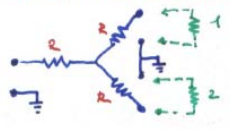
\includegraphics{./Immagini/Sdoppiatore.png}
\caption{Uno sdoppiatore di segnale ad alta frequenza}
\label{fig:sdoppiatore}
\end{center}
\end{figure}
\section{Trasformatore invertente}
Il trasformatore invertente, serve ad invertire la polarit\`a di segnali pi\`u brevi di 100 ns, in alternativa \`e necessario usare altri dispositivi ad-hoc, come gli amplificatori.
\begin{figure}[htbp]
\begin{center}
	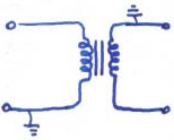
\includegraphics[scale=1.00]{./Immagini/TrasformatoreInvertente.png}
\caption{Un trasformatore invertente, il ramo dove \`e presente la messa a terra \`e invertito.}
\end{center}
\end{figure}
\section{La formatura del segnale}
Spesso \`e necessario formare un segnale, ovvero fare in moto che abbia determinati tempi di salita e di discesa dell'impulso,
questo pu\`o essere ottenuto con dispositivi passivi o attivi.
\subsection{Differenziatore CR o filtro passa-alto}
\begin{figure}[htbp]
\begin{center}
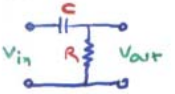
\includegraphics[scale=1]{./Immagini/FiltroCR.png}
\caption{Filtro passa-alto}
\label{fig:filtroCR}
\end{center}
\end{figure}
Il filtro passa-alto (fig.~\ref{fig:filtroCR}) pu\`o essere utilizzato per formare il fronte di discesa di un segnale:
all'aumentare della frequenza di taglio ($\propto \tau^{-1}=(RC)^{-1}$) la componente in bassa frequenza del segnale viene smorzata, lasciando solamente le alte frequenze che vanno a 0 pi\`u velocemente.
In conclusione al diminuire di $\tau$ il segnale aumenta la propria velocit\`a di smorzamento.
Questo filtro elimina la componente in bassa frequenza ($\omega \cdot \tau \ll 1$) del segnale, lasciando i segnali sinusoidali ad alta frequenza ($\omega \cdot \tau \gg 1$) inalterati.\\
Un segnale in uscita dal preamplificatore pu\`o essere approssimato con un gradino
\begin{equation*}
V_in(t) = \begin{cases}
0 \text{ se }t<0\\
V_0 \text{ se }t\ge 0
\end{cases}
\end{equation*}
in quanto possiede un fronte di salita molto veloce ed un fronte di discesa molto lento (quasi piatto).
Un segnale di questa forma che entra in un CR esce con questa formatura
\begin{equation*}
V_{out}(t) = V_0 e^{-t/\tau} 
\end{equation*}
ovvero con un fronte di discesa formato. 
Questo perch\`e il fronte di salita essendo veloce (quindi formato quasi unicamente da componenti ad alta frequenza) passa inalterato, mentre il fronte di discesa,
essendo lento (quindi formato quasi unicamente da armoniche a bassa frequenza), viene determinato da quali frequenze basse vengono fatte passare.
\subsection{Integratore RC o filtro passa-basso}
\begin{figure}[htbp]
\begin{center}
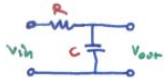
\includegraphics[scale=1]{./Immagini/FiltroRC.png}
\caption{Filtro passa-basso}
\label{fig:filtroRC}
\end{center}
\end{figure}
Il filtro passa-basso (fig.~\ref{fig:filtroRC}) pu\`o essere utilizzato per formare il fronte di salita di un segnale:
all'aumentare della frequenza di taglio ($\propto \tau^{-1}=(RC)^{-1}$) vengono ammesse nuove componenti ad alta frequenza che, avendo derivata maggiore, fanno salire il segnale pi\`u rapidamente.
In conclusione al diminuire di $\tau$ il segnale aumenta la propria velocit\`a di smorzamento.
Questo filtro elimina la componente in bassa frequenza ($\omega \cdot \tau \ll 1$) del segnale, lasciando i segnali sinusoidali ad alta frequenza ($\omega \cdot \tau \gg 1$) inalterati.\\
Un segnale in uscita dal preamplificatore pu\`o essere approssimato con un gradino
\begin{equation*}
V_in(t) = \begin{cases}
0 \text{ se }t<0\\
V_0 \text{ se }t\ge 0
\end{cases}
\end{equation*}
Un segnale di questa forma che entra in un RC esce con questa formatura
\begin{equation*}
V_{out}(t) = V_0 (1-e^{-t/\tau})
\end{equation*}
ovvero con un fronte di salita formato. 
Questo perch\`e il fronte di salita essendo veloce (quindi formato quasi unicamente da componenti ad alta frequenza) viene determinato da quali frequenze vengono ammesse,
mentre il fronte di discesa, essendo lento (quindi formato quasi unicamente da armoniche a bassa frequenza), passa inalterato.
\subsection{Formatura CR-RC}
Se io combino i due filtri precedentemente descritti frapponendo fra i due un amplificatore operazionale (fig~\ref{fig:filtroCRRC}) di disaccoppiamento con guadagno pari a 1,
si ottiene una catena di lettura in grado di formare sia il fronte di salita che il fronte di discesa dell'impulso.
\begin{figure}[htbp]
\begin{center}
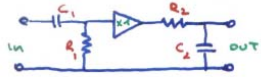
\includegraphics[scale=1]{./Immagini/FiltroCRRC.png}
\caption{Formatura tramite un CR-RC}
\label{fig:filtroCRRC}
\end{center}
\end{figure}
Se supponiamo di sottoporre la catena ad un gradino di tensione di ampiezza $V_0$ (approssima bene i segnali in uscita da un preamplificatore), in uscita si otterr\`a:
\begin{equation*}
V(t) = V_0 \, e^{-t/\tau_2}(1 - e^{-t/\tau_1}) 
\end{equation*}
Se $\tau_1 \approx \tau_2$ e sviluppando al primo ordine il termine tra parentesi si ottiene:
\begin{equation*}
V(t) = V_0 \, e^{-t / \tau} \frac{t}{\tau}
\end{equation*}
Il tempo caratteristico del RC (passa basso) determina il fronte di salita: diminuendo $\tau$ (=$RC$) aumenta la frequenza di taglio, per cui si allarga la banda di basse frequenze ammesse, aumentando la velocit\`a di salita.
Il tempo caratteristico del CR (passa alto) determina il fronte di discesa: se $\tau$ aumenta, la frequenza di taglio diminuisce, introducendo componenti a bassa frequenza che rallentano la discesa del segnale.
In conclusione aumentare $\tau_{RC}$ aumenta la velocit\`a di salita, aumentare $\tau_{CR}$ diminuisce la velocit\`a di discesa.\\
Le costanti di tempo devono essere scelte in modo tale da poter raccogliere le cariche disponibili, ridurre il rumore elettronico ed evitare il \textit{pile-up}.
In particolare alcune richieste sono in contrapposizione, ad esempio per essere sicuri di raccogliere tutte le cariche pu\`o essere utile avere un tempo di discesa lungo, 
tuttavia questo aumenta il rischio di avere del \textit{pile-up}. 
\begin{figure}[htbp]
\begin{center}
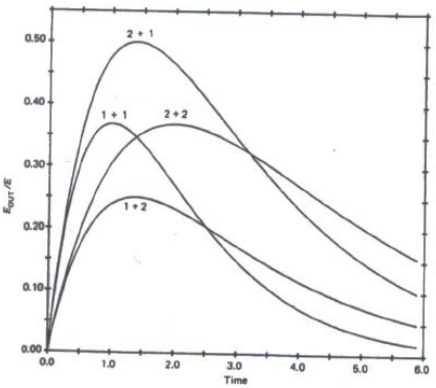
\includegraphics[scale=1]{./Immagini/FormaturaRCCR.png}
\caption{Esempi di segnali formati con varie costanti di tempo}
\label{fig:formaturaRCCR}
\end{center}
\end{figure}
\subsection{Formatura gaussiana}
Costruendo un circuito CR-(RC)$^n$ con n RC in cascata si pu\`o ottenere una formatura gaussiana dell'impulso:
\begin{equation}
V(t) = V_0 \, e^{-t/\tau} (1-e^{-t/\tau})^n \approx V_0 \left(\frac{t}{\tau}\right)^n e^{-t/\tau}
\end{equation}
Questa forma per $n>4$ approssima bene una gaussiana;
il massimo viene raggiunto in $n\tau$, detto anche \textit{\textbf{peaking time}}).
A parit\`a di \textit{peaking time}, questa formatura recupera la linea di base pi\`u velocemente rispetto alla formatura RC-CR.
Questa formatura \`e la migliore in qualit\`a di rapporto segnale-rumore.
\subsection{Formature con fitri attivi}
Utilizzando circuiti con elementi attivi come diodi o transistor si possono ottenere formature pi\`u fantasiose.
\begin{itemize}
\item \textbf{Formatura triangolare}, ottenibile con una serie di filtri attivi
\item \textbf{Formatura trapezoidale}, utilizzata se il risetime \`e variabile, in modo da avere tutta la carica raccolta in rivelatori con grande variabilit\`a di tempi di risposta.
Questa formatura viene ottenuta con circuiti analogici e digitali.
\end{itemize}
\subsection{Formatura CR-RC-CR}
Utilizzata per dare una forma bipolare all'impulso nel caso di rate molto elevati.
\subsection{Formatura con singola linea di ritardo}
La singola linea di ritardo (SDL) viene utilizzata per ridurre la durata di impulsi troppo lunghi:
un segnale viene sdoppiato in due rami, uno \`e il ramo di output, l'altro viene lasciato aperto.
Se il tempo di propagazione $\tau$ in quest'ultimo \`e molto maggiore del tempo di salita dell'impulso, allora dopo $2 \tau$ il segnale ritorna identico sulla linea di output, 
ma invertito.
Sommandosi al segnale precedente lo annulla.
\begin{figure}[htbp]
\begin{center}
	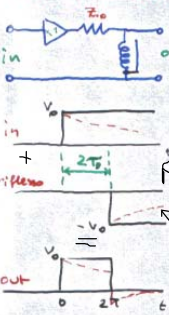
\includegraphics[scale=1]{./Immagini/SDL.png}
	\caption{Formatura con SDL (Single Delay Line)}
\label{fig:SDL}
\end{center}
\end{figure}
Nel caso il segnale avesse un tempo decadimento si pu\`o presentare il problema dell'\textit{undershoot} (tratteggio rosso nell'immagine): per risolverlo
\`e necessario attenuare in modo opportuno il segnale lungo la linea di ritardo.
\subsection{Formatura con doppia linea di ritardo}
\`E possibile rendere il segnale bipolare imponendo un'altra linea di ritardo in uscita dalla SDL con lo stesso tempo della prima linea.
Il problema di questa formatura \`e che non passa da filtri, per cui presenta il problema del rumore non filtrato, per questo viene usata prevalentemente
in rivelatori con poca risoluzione o per i segnali logici.
\section{Cancellazione del polo zero}
Nella realt\`a i nostri dispositivi non sono sottoposti a dei gradini, bensi a segnali che salgono molto velocemente e decadono molto lentamente.
I tempi di decadimento possono portare a degli \textit{undershoot} che vengono recuperati in tempi nell'ordine dei $\mu$s causando problemi nella forma degli
impulsi successivi. \\
Si dimostra che nei CR-RC il problema pu\`o essere risolto utilizzando una resistenza regolabile in parallelo alla capacit\`a nel CR.
\section{Spostamenti della linea di base}
Supponiamo di avere un treno di impulsi, poich\`e in un CR-RC la tensione media deve essere nulla, in caso di alti rate si pu\`o osservare uno spostamento
della linea di base in modo da mantenere tale media nulla.\\
Nel caso di impulsi identici equispaziati lo spostamento non \`e problematico in quanto costante, tuttavia nella realt\`a gli impulsi hanno forma diversa per cui lo spostamento
pu\`o risultare un problema.\\
Per risolvere il problema si pu\`o usare una formatura bipolare in modo da compensare questo effetto, tuttavia porta ad avere alti rapporti rumore-segnale.
Un'altra soluzione proviene dall'accoppiare il segnale in tensione continua che successivamente viene eliminato con un filtro.